\documentclass[11pt]{report}
\usepackage[a4paper, tmargin=2.54cm, bmargin=2.54cm, lmargin=3.17cm, rmargin=3.17cm]{geometry}
\newcommand{\head}[1]{\textnormal{\textbf{#1}}}

\usepackage{titlesec}    % Remove the text 'Chapter' from each chapter.
\titleformat{\chapter}{\normalfont\huge\bf}{\thechapter}{20pt}{\huge\bf}

\title{Master's thesis Health Informatics \the\year}
\author{authors}
\setcounter{tocdepth}{3}

\usepackage{graphicx}
\usepackage{booktabs}
\usepackage{natbib}
\usepackage{xcolor}
\usepackage[spanish, es-tabla]{babel}

%\usepackage{helvet}

%MORE PACKAGES HERE


\begin{document}

%%%%%%%%%%%%%%%%%%%%%%%%%%%%
%%% Cambiar 'Figura' por 'Imagen'
\renewcommand{\figurename}{Imagen}
\renewcommand{\listfigurename}{Lista de Imágenes}

%%%%%%%%%%%%%%%%%%%%%%%%%%%%
%%%% PORTADA
%%%%%%%%%%%%%%%%%%%%%%%%%%%%

\thispagestyle{empty}
\begin{titlepage}
    \hspace{-1.5cm}
	
\includegraphics[width=40mm]{img/LogoETSIIT.png}
	
\includegraphics[width=40mm]{img/LogoFacultadCiencias.jpeg}
	\hfill
	
\includegraphics[width=50mm]{img/LogoUGR.png}
	
	\noindent\begin{small} \sffamily
		\begin{minipage}{0.65\textwidth}
			Doble Grado en Ingeniería Informática y Matemáticas\\
			Curso 2021/2022\\
			Trabajo de Fin de Grado\\
		\end{minipage}
	\hrule
	\end{small}

	%Thesis title
	\vspace{1cm}
	{\LARGE\noindent \textbf{Fractales y Geometría Fractal} \par}
	\vspace{0.5cm}
	%Thesis subtitle
	{\Large\noindent Fractales, geometría fractal y aplicaciones en la ciencia. Visualización de fractales con Ray-Tracing \par}
	\vspace{2cm}
	%Author's name
	{\LARGE\noindent Autor: Juan Antonio Villegas Recio \par} %%%%% CHANGE STUDENT HERE

	\vfill
		
	\hrule
	\vspace{0.3cm}
	
%%% CHANGE SUPERVISORS AND REVIEWERS BELOW
	
	\begin{table}[h!]
		\begin{footnotesize} \sffamily
			\begin{tabular}{p{0.21\textwidth}p{0.79\textwidth}}
				Autor: & Juan Antonio Villegas Recio \\
				Tutor de Matemáticas:    & Manuel Ruiz Galán, Catedrático de Universidad\\
				& Departamento de Matemática Aplicada, Universidad de Granada \\
				Tutor de Informática:      & Carlos Ureña Almagro, Profesor Titular de Universidad \\
				& Departamento de Lenguajes y Sistemas Informáticos, Universidad de Granada
			\end{tabular}
		\end{footnotesize}
	\end{table}
	
\end{titlepage}

\newpage
%%%%%%%%%%%%%%%%%%%%%%%%%%%%

\chapter*{Affirmation}

%%%%%%%%%%%%%%%%%%%%%%%%%%%%
% ABSTRACT
%%%%%%%%%%%%%%%%%%%%%%%%%%%%

I hereby affirm that this Master thesis was composed by myself, that the work contained herein is my own except where explicitly stated otherwise in the text. This work has not been submitted for any other degree or professional qualification except as specified; nor has it been published. \\
\newline
City, date

\vspace{0cm}
\noindent
\includegraphics[width=0.3\textwidth]{img/mysignature.png}

\vspace*{-1.1cm}
\noindent \rule{0.3\textwidth}{.3pt}\\
\vspace{0.3cm}
\noindent \large{Student's name}        %%% CHANGE STUDENT'S NAME HERE


%%%%%%%%%%%%%%%%%%%%%%%%%%%%
% ABSTRACT
%%%%%%%%%%%%%%%%%%%%%%%%%%%%

\chapter*{Abstract}

\thispagestyle{empty}

\textit{\texttt{(no more than 250-300 words)}}

\subsection*{Background}
Describe background shortly

\subsection*{Aim}
Describe the aim of your study

\subsection*{Method}
Describe your methods

\subsection*{Results}
Describe the main results of your study

\subsection*{Conclusion}
State your conclusion

\subsection*{\emph{Keywords:}} No more than six keywords, preferably MeSH terms


\tableofcontents
\setcounter{page}{1}
\pagenumbering{roman}
\thispagestyle{plain}


%%%%%%%%%%%%%%%%%%%%%%%%%%%%
% LISTA DE ABREVIATURAS
%%%%%%%%%%%%%%%%%%%%%%%%%%%%

\chapter*{Lista de Abreviaturas}

%%%% En orden alfabético
\begin{itemize}
\item SDF: Signed Distance Function
\end{itemize}
\addcontentsline{toc}{chapter}{Lista de Abreviaturas}

%%%%%%%%%%%%%%%%%%%%%%%%%%%%
% LISTA DE IMÁGENES
%%%%%%%%%%%%%%%%%%%%%%%%%%%%
\listoffigures
\thispagestyle{plain}
\addcontentsline{toc}{chapter}{Lista de Imágenes}

%%%%%%%%%%%%%%%%%%%%%%%%%%%%
% LIST DE TABLAS
%%%%%%%%%%%%%%%%%%%%%%%%%%%%
\listoftables
\thispagestyle{plain}
\addcontentsline{toc}{chapter}{Lista de Tablas}
% \addtocontents{toc}{\bigskip}

%%%%%%%%%%%%%%%%%%%%%%%%%%%%
%%%%%%%%%%%%%%%%%%%%%%%%%%%%
% INICIO DEL TRABAJO
%%%%%%%%%%%%%%%%%%%%%%%%%%%%
%%%%%%%%%%%%%%%%%%%%%%%%%%%%

\chapter{Introducción}
\setcounter{page}{1}
\pagenumbering{arabic}


\section{Background}

This chapter offers an introduction to the thesis and typically introduces the problem, the research question and delimitations.

It can be nice to include figures already in this first chapter. A picture of a pipe is given in Figure \ref{fig:pipe}.

\begin{figure} [h]
\centering

\includegraphics[scale = 0.6]{img/pipe.jpg}
\caption{A Picture of a Pipe}
 \label{fig:pipe}
\end{figure}


\subsection{Use subheadings that fit your topic}
Lorem ipsum dolor sit amet, consectetur adipiscing elit, sed do eiusmod tempor incididunt ut labore et dolore magna aliqua. Ut enim ad minim veniam, quis nostrud exercitation ullamco laboris nisi ut aliquip ex ea commodo consequat. Duis aute irure dolor in reprehenderit in voluptate velit esse cillum dolore eu fugiat nulla pariatur. Excepteur sint occaecat cupidatat non proident, sunt in culpa qui officia deserunt mollit anim id est laborum.

Lorem ipsum dolor sit amet, consectetur adipiscing elit, sed do eiusmod tempor incididunt ut labore et dolore magna aliqua. Ut enim ad minim veniam, quis nostrud exercitation ullamco laboris nisi ut aliquip ex ea commodo consequat. Duis aute irure dolor in reprehenderit in voluptate velit esse cillum dolore eu fugiat nulla pariatur. Excepteur sint occaecat cupidatat non proident, sunt in culpa qui officia deserunt mollit anim id est laborum.

Lorem ipsum dolor sit amet, consectetur adipiscing elit, sed do eiusmod tempor incididunt ut labore et dolore magna aliqua. Ut enim ad minim veniam, quis nostrud exercitation ullamco laboris nisi ut aliquip ex ea commodo consequat. Duis aute irure dolor in reprehenderit in voluptate velit esse cillum dolore eu fugiat nulla pariatur. Excepteur sint occaecat cupidatat non proident, sunt in culpa qui officia deserunt mollit anim id est laborum.

At vero eos et accusamus et iusto odio dignissimos ducimus qui blanditiis praesentium voluptatum deleniti atque corrupti quos dolores et quas molestias excepturi sint occaecati cupiditate non provident, similique sunt in culpa qui officia deserunt mollitia animi, id est laborum et dolorum fuga. Et harum quidem rerum facilis est et expedita distinctio. Nam libero tempore, cum soluta nobis est eligendi optio cumque nihil impedit quo minus id quod maxime placeat facere possimus, omnis voluptas assumenda est, omnis dolor repellendus. Temporibus autem quibusdam et aut officiis debitis aut rerum necessitatibus saepe eveniet ut et voluptates repudiandae sint et molestiae non recusandae. Itaque earum rerum hic tenetur a sapiente delectus, ut aut reiciendis voluptatibus maiores alias consequatur aut perferendis doloribus asperiores repellat.

\section{Problem description}

Lorem ipsum dolor sit amet, consectetur adipiscing elit, sed do eiusmod tempor incididunt ut labore et dolore magna aliqua. Ut enim ad minim veniam, quis nostrud exercitation ullamco laboris nisi ut aliquip ex ea commodo consequat. Duis aute irure dolor in reprehenderit in voluptate velit esse cillum dolore eu fugiat nulla pariatur. Excepteur sint occaecat cupidatat non proident, sunt in culpa qui officia deserunt mollit anim id est laborum.

\section{Aim}

Lorem ipsum dolor sit amet, consectetur adipiscing elit, sed do eiusmod tempor incididunt ut labore et dolore magna aliqua. Ut enim ad minim veniam, quis nostrud exercitation ullamco laboris nisi ut aliquip ex ea commodo consequat. Duis aute irure dolor in reprehenderit in voluptate velit esse cillum dolore eu fugiat nulla pariatur. Excepteur sint occaecat cupidatat non proident, sunt in culpa qui officia deserunt mollit anim id est laborum.

\section{Objectives}

Lorem ipsum dolor sit amet, consectetur adipiscing elit, sed do eiusmod tempor incididunt ut labore et dolore magna aliqua. Ut enim ad minim veniam, quis nostrud exercitation ullamco laboris nisi ut aliquip ex ea commodo consequat. Duis aute irure dolor in reprehenderit in voluptate velit esse cillum dolore eu fugiat nulla pariatur. Excepteur sint occaecat cupidatat non proident, sunt in culpa qui officia deserunt mollit anim id est laborum.

\section{Research questions}

Lorem ipsum dolor sit amet, consectetur adipiscing elit, sed do eiusmod tempor incididunt ut labore et dolore magna aliqua. Ut enim ad minim veniam, quis nostrud exercitation ullamco laboris nisi ut aliquip ex ea commodo consequat. Duis aute irure dolor in reprehenderit in voluptate velit esse cillum dolore eu fugiat nulla pariatur. Excepteur sint occaecat cupidatat non proident, sunt in culpa qui officia deserunt mollit anim id est laborum.



\chapter{Methods}

This chapter is about methodology and discusses research strategies, data collection methods and data analysis methods. A simple overview of the relationships between these is given in Figure \ref{fig:methods}.


\begin{figure} [h]
\centering
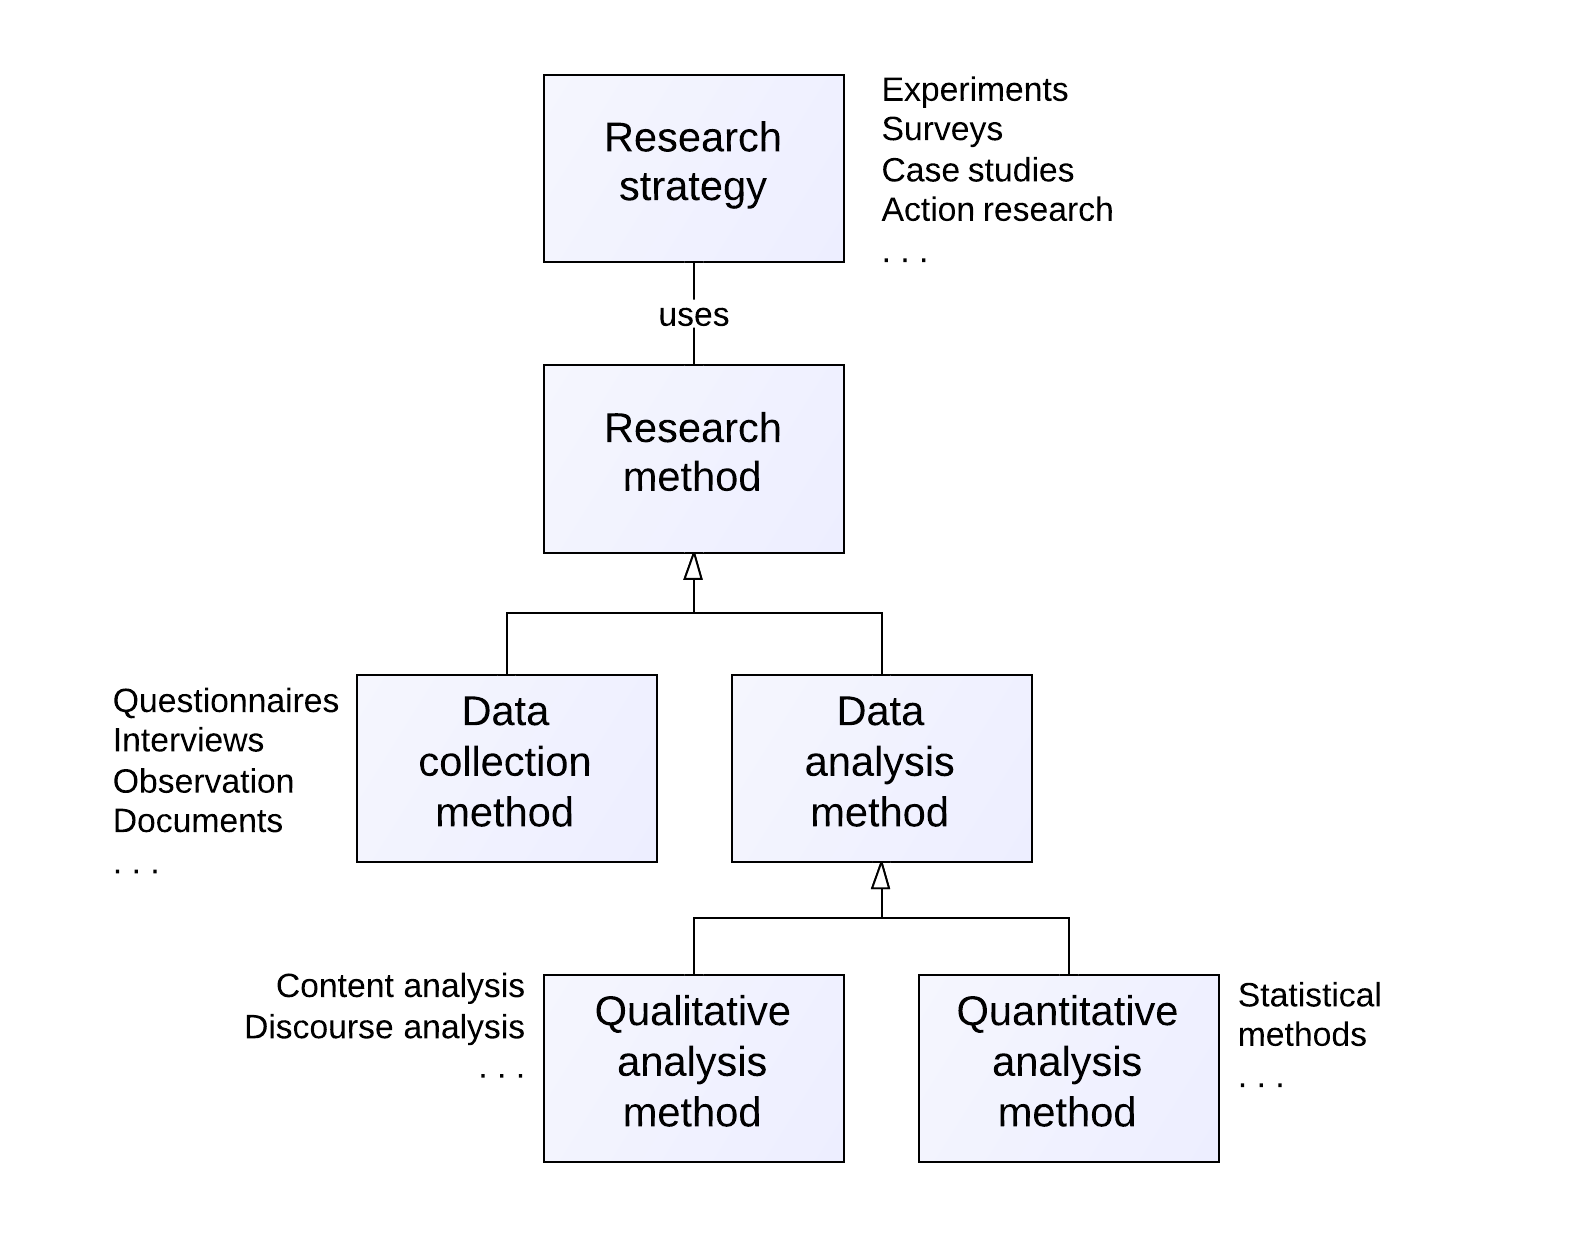
\includegraphics[scale = 0.2]{img/methods.png}
\caption{Research Strategies and Research Methods}
 \label{fig:methods}
\end{figure}

\section{Research approach/study design}

Lorem ipsum dolor sit amet, consectetur adipiscing elit, sed do eiusmod tempor incididunt ut labore et dolore magna aliqua. Ut enim ad minim veniam, quis nostrud exercitation ullamco laboris nisi ut aliquip ex ea commodo consequat. Duis aute irure dolor in reprehenderit in voluptate velit esse cillum dolore eu fugiat nulla pariatur. Excepteur sint occaecat cupidatat non proident, sunt in culpa qui officia deserunt mollit anim id est laborum.

\section{Study setting}

Lorem ipsum dolor sit amet, consectetur adipiscing elit, sed do eiusmod tempor incididunt ut labore et dolore magna aliqua. Ut enim ad minim veniam, quis nostrud exercitation ullamco laboris nisi ut aliquip ex ea commodo consequat. Duis aute irure dolor in reprehenderit in voluptate velit esse cillum dolore eu fugiat nulla pariatur. Excepteur sint occaecat cupidatat non proident, sunt in culpa qui officia deserunt mollit anim id est laborum.

\section{Data collection}

Lorem ipsum dolor sit amet, consectetur adipiscing elit, sed do eiusmod tempor incididunt ut labore et dolore magna aliqua. Ut enim ad minim veniam, quis nostrud exercitation ullamco laboris nisi ut aliquip ex ea commodo consequat. Duis aute irure dolor in reprehenderit in voluptate velit esse cillum dolore eu fugiat nulla pariatur. Excepteur sint occaecat cupidatat non proident, sunt in culpa qui officia deserunt mollit anim id est laborum.

\section{Data analysis}

Lorem ipsum dolor sit amet, consectetur adipiscing elit, sed do eiusmod tempor incididunt ut labore et dolore magna aliqua. Ut enim ad minim veniam, quis nostrud exercitation ullamco laboris nisi ut aliquip ex ea commodo consequat. Duis aute irure dolor in reprehenderit in voluptate velit esse cillum dolore eu fugiat nulla pariatur. Excepteur sint occaecat cupidatat non proident, sunt in culpa qui officia deserunt mollit anim id est laborum.

\section{Ethical considerations}

Lorem ipsum dolor sit amet, consectetur adipiscing elit, sed do eiusmod tempor incididunt ut labore et dolore magna aliqua. Ut enim ad minim veniam, quis nostrud exercitation ullamco laboris nisi ut aliquip ex ea commodo consequat. Duis aute irure dolor in reprehenderit in voluptate velit esse cillum dolore eu fugiat nulla pariatur. Excepteur sint occaecat cupidatat non proident, sunt in culpa qui officia deserunt mollit anim id est laborum.


\chapter{Results}


This chapter can present the results of the study. Tables are often helpful for presenting results. For example, have a look at Table \ref{tab:titles1}.

\begin {table} [h]
\begin{tabular}{ccc}
\hline
\head{Author} & \head{Title} & \head{Publication Year}\\
\hline
\verb|Gottlob Frege| & \verb|Begriffsschrift| & \rmfamily 1879
\\
\verb|Bertrand Russell| & \verb|Principia Mathematica| & \sffamily 1910
\\
\verb|Ludwig Wittgenstein| & \verb|Philosophical Investigations| & \ttfamily 1953\\
\hline
\end{tabular}
\caption {Philosophical Titles 1} \label{tab:titles1} 
\end{table}

The same data are shown in Table \ref{tab:titles2} but with different formatting.

\begin {table} [h] 
\begin{tabular}{lll}
\toprule[1.5pt]
\head{Author} & \head{Title} & \head{Publication Year}\\
\midrule
\verb|Gottlob Frege| & \verb|Begriffsschrift| & \rmfamily 1879
\\
\verb|Bertrand Russell| & \verb|Principia Mathematica| & \sffamily 1910
\\
\verb|Ludwig Wittgenstein| & \verb|Philosophical Investigations| & \ttfamily 1953\\
\bottomrule[1.5pt] 
\end{tabular}
\caption {Philosophical Titles 2} \label{tab:titles2}
\end{table}


\section{Subheading}

Lorem ipsum dolor sit amet, consectetur adipiscing elit, sed do eiusmod tempor incididunt ut labore et dolore magna aliqua. Ut enim ad minim veniam, quis nostrud exercitation ullamco laboris nisi ut aliquip ex ea commodo consequat. Duis aute irure dolor in reprehenderit in voluptate velit esse cillum dolore eu fugiat nulla pariatur. Excepteur sint occaecat cupidatat non proident, sunt in culpa qui officia deserunt mollit anim id est laborum.

\section{Subheading}

Lorem ipsum dolor sit amet, consectetur adipiscing elit, sed do eiusmod tempor incididunt ut labore et dolore magna aliqua. Ut enim ad minim veniam, quis nostrud exercitation ullamco laboris nisi ut aliquip ex ea commodo consequat. Duis aute irure dolor in reprehenderit in voluptate velit esse cillum dolore eu fugiat nulla pariatur. Excepteur sint occaecat cupidatat non proident, sunt in culpa qui officia deserunt mollit anim id est laborum.


\chapter{Discussion}

This chapter could discuss your work. Comparing the results of your work to those of  previous studies is one important part of the discussion. See how this can be done in 
\cite{Simon1996-hh} and \cite{Hevner2004-wq}.

\section{Subheading}

Lorem ipsum dolor sit amet, consectetur adipiscing elit, sed do eiusmod tempor incididunt ut labore et dolore magna aliqua. Ut enim ad minim veniam, quis nostrud exercitation ullamco laboris nisi ut aliquip ex ea commodo consequat. Duis aute irure dolor in reprehenderit in voluptate velit esse cillum dolore eu fugiat nulla pariatur. Excepteur sint occaecat cupidatat non proident, sunt in culpa qui officia deserunt mollit anim id est laborum.

\section{Subheading}

Lorem ipsum dolor sit amet, consectetur adipiscing elit, sed do eiusmod tempor incididunt ut labore et dolore magna aliqua. Ut enim ad minim veniam, quis nostrud exercitation ullamco laboris nisi ut aliquip ex ea commodo consequat. Duis aute irure dolor in reprehenderit in voluptate velit esse cillum dolore eu fugiat nulla pariatur. Excepteur sint occaecat cupidatat non proident, sunt in culpa qui officia deserunt mollit anim id est laborum.

\chapter{Conclusion}

Lorem ipsum dolor sit amet, consectetur adipiscing elit, sed do eiusmod tempor incididunt ut labore et dolore magna aliqua. Ut enim ad minim veniam, quis nostrud exercitation ullamco laboris nisi ut aliquip ex ea commodo consequat. Duis aute irure dolor in reprehenderit in voluptate velit esse cillum dolore eu fugiat nulla pariatur. Excepteur sint occaecat cupidatat non proident, sunt in culpa qui officia deserunt mollit anim id est laborum.

\textbf{Note about referencing:} \textit{In LaTex, literature references are handled by creating a BibTeX file and referring to it. From Google Scholar, you can grab BibTeX references by clicking on "Import into BibTeX" below a search result. You can also generate BibTeX files from reference managers, such as Mendeley, Paperpile or Zotero.}


%%%%%%%%%%%%%%%%%%%%%%%%%%%%
% REFERENCES
%%%%%%%%%%%%%%%%%%%%%%%%%%%%

\bibliographystyle{agsm}
\bibliography{references}
% \addtocontents{toc}{\bigskip}
\addcontentsline{toc}{part}{Bibliography}


%%%%%%%%%%%%%%%%%%%%%%%%%%%%
% APPENDICES
%%%%%%%%%%%%%%%%%%%%%%%%%%%%

\appendix
\cleardoublepage
% \addtocontents{toc}{\bigskip}
\addcontentsline{toc}{part}{Appendices}

%% OPTIONAL - Max 10-15 pages in total

\chapter{Appendix title}

\chapter{Another Appendix}

\end{document}